\documentclass[12pt, twoside]{article}
%\documentclass[12pt, twoside]{article}
\usepackage[letterpaper, margin=1in, headsep=0.2in]{geometry}
\setlength{\headheight}{0.6in}
%\usepackage[english]{babel}
\usepackage[utf8]{inputenc}
\usepackage{microtype}
\usepackage{amsmath}
\usepackage{amssymb}
%\usepackage{amsfonts}
\usepackage[nomessages]{fp} %\FPeval{\var-name}{2*sin(pi/6)}
\usepackage{siunitx} %units in math. eg 20\milli\meter
\usepackage{yhmath} % for arcs, overparenth command
\usepackage{tikz} %graphics
\usetikzlibrary{quotes, angles, arrows, arrows.meta}
\usepackage{pgfplots}
\usepgfplotslibrary{fillbetween}
\pgfplotsset{compat=1.16}
\usepackage{graphicx} %consider setting \graphicspath{{images/}}
\usepackage{parskip} %no paragraph indent
\usepackage{enumitem}
\usepackage{multicol}
\usepackage{venndiagram}

\usepackage{fancyhdr}
\pagestyle{fancy}
\fancyhf{}
\renewcommand{\headrulewidth}{0pt} % disable the underline of the header
\raggedbottom
\hfuzz=2mm %suppresses overfull box warnings

\usepackage{hyperref}

\fancyhead[LE]{\thepage}
\fancyhead[RO]{Markscheme}
\fancyhead[LO]{La Scuola d'Italia / Dr.\ Huson / IB Math 11 \\* 18 November 2026}

\begin{document}
\subsubsection*{4.1 Homework: Quadratic Functions --- Markscheme}

\emph{Total: 54 marks.}

\begin{enumerate}[itemsep=0.3cm]

%--- Problem 1 [14 marks] ---
\item[1.] [Maximum mark: 14]

\textbf{(a)} (i) $c = -15$, from the standard form \hfill \textbf{A1}

(ii) $p = -1$, \ $q = 5$, from the factored form \hfill \textbf{A1}

(iii) $h = 2$, \ $k = -27$, from the vertex form \hfill \textbf{A1}

\emph{Each answer must be written as an equation naming the coefficient.
Accept $(0, -15)$; $(-1, 0)$ and $(5, 0)$; $(2, -27)$ together with the
coefficient names. Accept $p = 5$, $q = -1$. Common error: $p = 1$,
$q = -5$ or $h = -2$, the signs read straight from the brackets: A0.}

\begin{center}
\begin{tikzpicture}
\begin{axis}[axis lines=middle, xlabel={$x$}, ylabel={$y$},
  xmin=-2.5, xmax=6.5, ymin=-31, ymax=6,
  xtick={-2,-1,...,6}, ytick={-30,-20,-10},
  width=8cm, height=8cm, samples=100]
  \addplot[thick, domain=-1.25:5.25] {3*(x-2)^2 - 27};
  \node[circle, fill, inner sep=1.5pt] at (axis cs:0,-15) {};
  \node[anchor=west] at (axis cs:0.3,-12) {$(0,\ -15)$};
  \node[circle, fill, inner sep=1.5pt] at (axis cs:-1,0) {};
  \node[circle, fill, inner sep=1.5pt] at (axis cs:5,0) {};
  \node[circle, fill, inner sep=1.5pt] at (axis cs:2,-27) {};
  \node[anchor=west] at (axis cs:2.2,-27.5) {$(2,\ -27)$};
\end{axis}
\end{tikzpicture}
\end{center}

Concave-up parabola through the three labelled points \hfill \textbf{A1}

$y$-intercept, both $x$-intercepts and the vertex labelled \hfill \textbf{A1}

\emph{FT from (i)--(iii).}

\textbf{(b)} $x = -\dfrac{-12}{2(3)}$ \hfill \textbf{M1}

$x = 2$ \hfill \textbf{A1}

$\dfrac{-1 + 5}{2} = 2$, the midpoint of the $x$-intercepts \hfill \textbf{R1}

\emph{The answer must be an equation, $x = 2$. Wrong method:
$-\frac{b}{2a}$ with $b = 12$ gives $x = -2$: M0A0.}

\textbf{(c)} $f(x) \ge -27$ \hfill \textbf{A1}

\emph{Accept $y \ge -27$ or $[-27, \infty[$. Do not accept $x \ge -27$ or
$f(x) > -27$.}

\textbf{(d)} $a = 3 > 0$, so the graph is concave up and narrower than
$y = x^{2}$ \hfill \textbf{A1}

Vertical stretch, scale factor $3$ \hfill \textbf{A1}

then a translation by the vector $\begin{pmatrix} 2 \\ -27 \end{pmatrix}$ \hfill \textbf{A1}

\emph{Accept ``right $2$, down $27$''. The stretch comes first: a translation
first, then the stretch, gives $3(x - 2)^{2} - 81$. Award the second A1
only for the correct order or a correct description of the order.}

\textbf{(e)} $3(x - 2)^{2} - 27 = 3(x^{2} - 4x + 4) - 27 = 3x^{2} - 12x + 12 - 27 = 3x^{2} - 12x - 15$ \hfill \textbf{A1}

$3(x + 1)(x - 5) = 3(x^{2} - 4x - 5) = 3x^{2} - 12x - 15$ \hfill \textbf{A1}

\emph{Answer given (AG): the expansion must be seen. Common error:
$3(x - 2)^{2} = (3x - 6)^{2}$, squaring the $3$: A0.}

\newpage

%--- Problem 2 [12 marks] ---
\item[2.] [Maximum mark: 12]

\textbf{(a)} $(1,\ 9)$ \hfill \textbf{A1}

maximum, since $a = -1 < 0$ \hfill \textbf{A1}

\textbf{(b)} $-(x^{2} - 2x + 1) + 9$ \hfill \textbf{M1}

$= -x^{2} + 2x + 8$ \hfill \textbf{A1}

\emph{Common error: $-x^{2} - 2x + 1 + 9$, the negative applied to $x^{2}$
only: M1A0.}

\textbf{(c)} $-(x^{2} - 2x - 8)$ \hfill \textbf{M1}

$= -(x - 4)(x + 2)$ \hfill \textbf{A1}

$x = -2$ and $x = 4$ \hfill \textbf{A1}

\emph{Accept $(4 - x)(x + 2)$ or $-(x + 2)(x - 4)$. FT from (b). Check: the
intercepts are $1 \pm 3$, three units either side of the axis $x = 1$.}

\textbf{(d)}

\begin{center}
\begin{tikzpicture}
\begin{axis}[axis lines=middle, xlabel={$x$}, ylabel={$y$},
  xmin=-3.5, xmax=5.5, ymin=-1.5, ymax=11,
  xtick={-3,-2,...,5}, ytick={2,4,6,8},
  width=8cm, height=8cm, samples=100]
  \addplot[thick, domain=-2.1:4.1] {-(x-1)^2 + 9};
  \node[circle, fill, inner sep=1.5pt] at (axis cs:1,9) {};
  \node[anchor=south west] at (axis cs:1.1,9) {$(1,\ 9)$};
  \node[circle, fill, inner sep=1.5pt] at (axis cs:0,8) {};
  \node[circle, fill, inner sep=1.5pt] at (axis cs:-2,0) {};
  \node[circle, fill, inner sep=1.5pt] at (axis cs:4,0) {};
\end{axis}
\end{tikzpicture}
\end{center}

Concave-down parabola, symmetric about $x = 1$ \hfill \textbf{A1}

vertex at $(1, 9)$ \hfill \textbf{A1}

$x$-intercepts $-2$ and $4$, $y$-intercept $8$ \hfill \textbf{A1}

\emph{FT from (a) and (c).}

\textbf{(e)} Reflection in the $x$-axis \hfill \textbf{A1}

then a translation by the vector $\begin{pmatrix} 1 \\ 9 \end{pmatrix}$ \hfill \textbf{A1}

\emph{Order matters: translating first and then reflecting gives
$-(x - 1)^{2} - 9$. Accept ``right $1$, up $9$''.}

\newpage

%--- Problem 3 [9 marks] ---
\item[3.] [Maximum mark: 9]

\textbf{(a)}

\begin{center}
\renewcommand{\arraystretch}{1.5}
\begin{tabular}{|l|c|c|c|c|}
\hline
 & $a$ & $b$ & $c$ & $\Delta = b^{2} - 4ac$ \\
\hline
Graph 1 & negative & positive & positive & positive \\
\hline
Graph 2 & positive & positive & positive & zero \\
\hline
\end{tabular}
\end{center}

\hfill \textbf{A1} for each correct cell (\textbf{A8})

\emph{Reasons: $a$ from the concavity (Graph 1 opens down, Graph 2 opens up);
$c$ is the $y$-intercept; $\Delta$ from the number of $x$-intercepts (two
for Graph 1, one, touching, for Graph 2); $b$ from the axis of symmetry
$x = -\frac{b}{2a}$. In Graph 2 the axis is left of the $y$-axis and
$a > 0$, so $b > 0$.}

\textbf{(b)} The axis of symmetry $x = -\dfrac{b}{2a}$ is to the right of
the $y$-axis, so $-\dfrac{b}{2a} > 0$. Since $a < 0$, $2a < 0$, so $b$ must
be positive. \hfill \textbf{R1}

\emph{The R1 needs both facts: the axis is at a positive $x$-value, and
$a$ is negative. Accept an equivalent argument: the graph is increasing as
it crosses the $y$-axis, so the gradient there, $b$, is positive.}

\bigskip \hrule \bigskip

%--- Problem 4 [9 marks] ---
\item[4.] [Maximum mark: 9]

\textbf{(a)} $y = a(x + 1)(x - 5)$ \hfill \textbf{M1}

$10 = a(0 + 1)(0 - 5)$, \quad $-5a = 10$ \hfill \textbf{M1}

$a = -2$, \quad $y = -2(x + 1)(x - 5)$ \hfill \textbf{A1}

\emph{Common error: $y = (x + 1)(x - 5)$ with no $a$, which has
$y$-intercept $-5$, not $10$: M1M0A0.}

\textbf{(b)} $-2(x^{2} - 4x - 5)$ \hfill \textbf{M1}

$y = -2x^{2} + 8x + 10$ \hfill \textbf{A1}

\emph{Check: $c = 10$ is the $y$-intercept. FT from (a).}

\textbf{(c)} $x = \dfrac{-1 + 5}{2} = 2$ \hfill \textbf{A1}

$y = -2(2 + 1)(2 - 5)$ \hfill \textbf{M1}

vertex $(2,\ 18)$ \hfill \textbf{A1}

range $y \le 18$ \hfill \textbf{A1}

\emph{Accept $x = -\frac{8}{2(-2)} = 2$. FT from (a) or (b).}

\newpage

%--- Problem 5 (GDC) [10 marks] ---
\item[5.] [Maximum mark: 10]

\textbf{(a)} Attempt to find the intersection of the two graphs \hfill \textbf{M1}

$(2.61,\ 90.6)$ \ $(2.60508\ldots,\ 90.6305\ldots)$ \hfill \textbf{A1}

$(14.4,\ 161)$ \ $(14.3949\ldots,\ 161.369\ldots)$ \hfill \textbf{A1}

\emph{GDC: Graphs app, f1(x) $= 40x - 2x^{2}$, f2(x) $= 6x + 75$, window
$0 \le x \le 20$, $0 \le y \le 220$; Menu, Analyze Graph, Intersection.
Accept an algebraic method: $2x^{2} - 34x + 75 = 0$, solved by the formula
or Polynomial Tools. The answers must be coordinates; $x$-values alone earn
M1A1A0.}

\textbf{(b)} $2.61 < x < 14.4$ \hfill \textbf{A1A1}

\emph{A1 for the two end values, A1 for the interval between them (the
revenue graph is above the cost graph). Accept $\le$. FT from (a).}

\textbf{(c)} $P(x) = 40x - 2x^{2} - (6x + 75)$ \hfill \textbf{M1}

$P(x) = -2x^{2} + 34x - 75$ \hfill \textbf{A1}

\emph{Common error: $-2x^{2} + 34x + 75$, the negative not applied to the
whole cost: M1A0.}

\textbf{(d)} $x = -\dfrac{34}{2(-2)} = 8.5$ \hfill \textbf{M1}

$850$ bicycle lights \hfill \textbf{A1}

$P(8.5) = 69.5$, so the maximum profit is $69\,500$ euros \hfill \textbf{A1}

\emph{Accept GDC: graph $P$, Menu, Analyze Graph, Maximum. Accept $x = 8.5$
for the first A1 only if the units are clear (hundreds). Wrong method: the
vertex of $R$, $x = 10$ and $R = 200$, maximises revenue, not profit:
M0A0A0. FT from (c).}

\end{enumerate}
\end{document}
